\thispagestyle{empty}
% FG & SRH
%Object space imaging and phase characterisation results.

Several bench top tests were performed to quantify the performance of the interferometer multi-path issues, . These tests fall into  , and tests for consistency between the sawtooth and sinusoidal source modulation.

\subsection{Interference tests}
To test the performance of the interferometer, the interferograms were recorded with both the probe and reference arm open, only the probe arm open and only the reference arm open.
For the cases where a single arm is open, only a DC offset should be observed in the detector signals; however, the presence of unwanted reflections (multi-path) within the system gives rise to interference, which leads to errors when both arms are open.
The extent of these problems is examined by checking the RMS of the AC component of the detector outputs, with various arms open (figure~\ref{fig:RMS_interference}).

\begin{figure}[!h]
\begin{center}
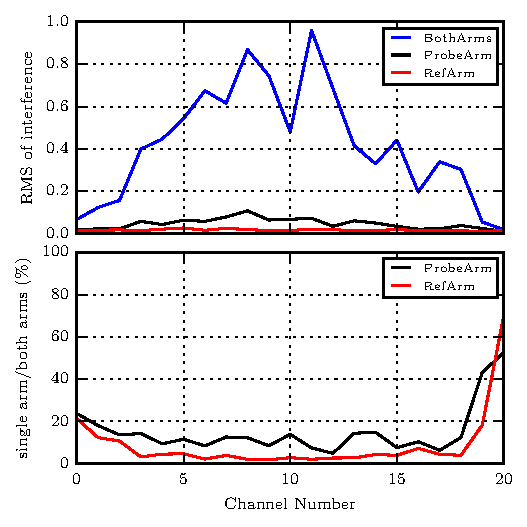
\includegraphics[]{figures/interference.pdf}
\end{center}
\caption{(a) RMS of the interferograms with various interferometer arms open for all of the interferometer channels. The variation in the amplitude with channel is due to different detector sensitivities and the Gaussian shape of the beam. (b) Ratio of the RMS from the single arms to both arms, highlighting the extent to which multi-path is a problem for each channel.}
\label{fig:RMS_interference}
\end{figure}

\subsection{Imaging Tests}
Stainless steel mirrors were manufactured with shallow sine waves machined into their surface to act as phase objects.
The wavelength and peak to peak depth of the sine waves for the different mirrors were: (wavelength$~=100\mathrm{mm}$,depth$~=1\mathrm{mm}$), ($100\mathrm{mm}$,$0.5\mathrm{mm}$), and ($60\mathrm{mm}$,$0.5\mathrm{mm}$).
The machining tollerance of these mirrors was measured to be within $10\mu\mathrm{m}$.
By placing these mirrors on a motorised vertical stage in the imaging plane, the imaging behaviour of the interferometer can be tested.
Figure~\ref{fig:moving_mirror_contour} shows one such tests with the ($100\mathrm{mm}$,$1\mathrm{mm}$) mirror, where at $t\approx5\mathrm{s}$ the mirror starts moving upwards, at $t\approx24\mathrm{s}$ the motorised stage stops before moving back downwards at $t\approx29\mathrm{s}$ (note the image is inverted at the detector array).

\begin{figure}[!h]
\begin{center}
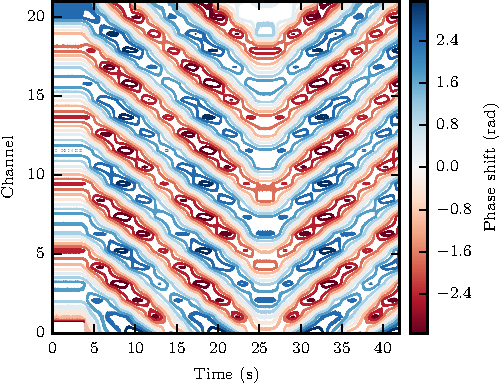
\includegraphics[]{figures/shot-85368-wavelength-100-depth-1-00pi-contour.pdf}
\end{center}
\caption{}
\label{fig:moving_mirror_contour}
\end{figure}

As the mirror moves vertically, the demodulated output from the $i^{\mathrm{th}}$ detector can be modelled as:
\begin{equation}
\label{eqn:wobbly_mirror_fit}
p_i(t) = A_i \sin(k x_i - \omega t + \phi)~~,
\end{equation}
where $\phi$ is an initial phase offset due to the starting position of the mirror, $A_i$ is the depth of modulation observed by the detector which should be the same across all channels, $k$ is the wavenumber of the sinusoidal modulation machined into the mirrors including any magnification due to the imaging system, $\omega$ is a function of the wavelength of the mirror and how quickly the motorised stage is moving, and the detectors location is given by $x_i$.

The demodulated signal from each channel should reproduce the sine that is created due to the path length change as the mirror moves upwards.
Additionally, each channel will see an initial phase in the sine wave, with the relationship between these initial phases across the channels representing the spatial structure of the wobbly mirror. 
Figure~\ref{fig:moving_mirror_amp_phase} shows the amplitudes and initial phases for the three different phase objects. 
The variation in the observed amplitude between the different channels is due to the multi path issues that have been described earlier.

\begin{figure}[!h]
\begin{center}
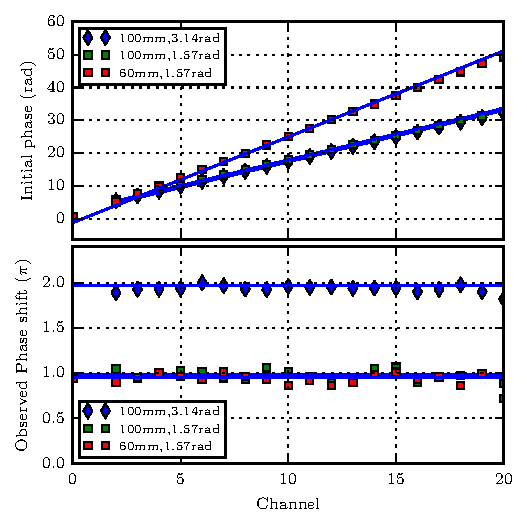
\includegraphics[]{figures/85368_85372_85391_k-amp.pdf}
\end{center}
\caption{(a) Plot of the initial phase for vertically subsequent detectors ($kx_i$ in equation~\protect\ref{eqn:wobbly_mirror_fit}). As the $k$ of a particular wobbly mirror is fixed, and $x_i$ are evenly spaced, the values are expected to form a straight line. The solid lines show the expected trend based on the dimensions of the mirrors and the speed of the stage. (b) Plots of $A_i$ to check for consistency in the observed depth across the detector channels.}
\label{fig:moving_mirror_amp_phase}
\end{figure}

To test the depth of field of the imaging system, the location of the wobbly mirror is moved through the focal plane, with measurements of the observed depth of the sinusoidal modulation recorded across all of the channels at specific discrete locations.
Figure~\ref{fig:depth_of_field} demonstrates that is a strong maximum in the data as the mirror approaches the focal plane demonstrating the imaging....
\begin{figure}[!h]
\begin{center}
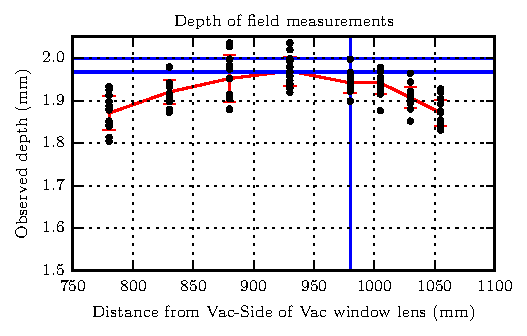
\includegraphics[]{figures/depth_of_field.pdf}
\end{center}
\caption{}
\label{fig:depth_of_field}
\end{figure}

